% This will be the quick overview/background to Cloud

%How we get the data (django and REST APIs), what we do with the data (database, analytics), and how we present it (website, phone)

We developed a web server application to serve as the primary coordinator of the system.
The server has several key responsibilities: exchanging information with SPOT sensors and user's smart phones, managing our database, and implementing a user account and billing system.
It must also serve a public-facing website for drivers and lot managers, perform real-time and historical data analytics, and provide endpoints to access the calculated data.

In order achieve these goals we relied primarily on the Django web framework and Django REST Framework library running on a Google App Engine instance.
Django is a web and REST framework written in Python which provides the backbone of our system including API endpoint generation for mobile, web, and sensors, user account management, data analytics, and real-time SPOT tracking.
The Google App Engine platform allows us to quickly and easily deploy web server code that is accessible from anywhere via an Internet connection with near-limitless scalability, automatic load balancing, and near 100\% up-time.

%%%%%%%%%%%%%%%%%%%%%%%%%%
\subsection{Setup Tutorial}
Our primary guide for setting up the development environment came from Google themselves.\footnote{https://cloud.google.com/python/django/appengine}
This tutorial walks through setting up the project instance on GCloud and commands needed to deploy our code to the server.
It also outlines the packages and libraries needed to run the server locally.
Additionally Google provides an SQL proxy application which allows your locally-running server to use the GCloud MySQL instance, which allowed us to share one database between team members and collaborate using common data.

We also utilized Visual Studio Code\footnote{https://code.visualstudio.com/}, a new IDE by Microsoft aimed at web application development.  On top of all the usual features like code completion and file management it also provides debugging and breakpoint services for both our Python and JavaScript code.
Using VSCode was incredibly helpful for development and did not require any additional configuration, it has predefined setting profiles for Django built in.

%%%%%%%%%%%%%%%%%%%%%%%%%%
\subsection{Back-end}

\subsubsection{Django}
Django is a web framework platform which follows the Model-View-Template pattern.
We used version 1.10.5, the latest stable release available that the Google App Engine officially supported.\footnote{https://docs.djangoproject.com/en/1.10/}
Throughout the development process there were not any major changes between versions that warranted upgrading.
\begin{itemize}

\item A Model refers to the database abstraction layer Django provides which allows developers to interact with a database in a purely Pythonic manner using dictionary like classes, there is no need to manually write SQL queries.
\item A View is the Python function which is called when an HTTP request is sent to the server.
Within this view parameters are parsed and analyzed, database exchanges are made, logic is performed, and output is determined.  The URL being requested can be parsed in order to determine which view should be called on the request.
\item A Template is used to deliver HTTP content as a response to the sender. 
A template contains both HTML markup and Python code. 
When the template is rendered by the View, the Python code is evaluated and a final HTML file is replied to the sender.
\end{itemize}
  

When a client makes an HTTP request to the server it can be in one of two forms: a GET or a POST message.
A GET message is used to request certain information from the server and does not alter any information on the server's side.
The GET message can specify parameters to narrow down the scope of data being requested.
For example a web client might submit a GET request for a specific user's parking status and use that user's email address as a parameter to the request.
A POST message is used to submit new or updated information to the server.
A POST message can also specify parameters to narrow the scope of data that it is updating.
For example, SPOT sensors submit a new POST request with their UUID as a parameter whenever they detect a car arriving or leaving.

Using Django allowed us to quickly and easily deploy new endpoints for the sensors, phones, and website to interact with as well as implement complex relational models and analytics.

%TODO overview of the apps we used


\subsubsection{Django REST Framework} %How JSON works and provides an easy way to transmit arbitrary data structures
On top of the standard Django framework we deployed the Django Representational State Transfer Framework (DRF) version 3.5.4 library to facilitate arbitrary client-server data exchanges in a programmatic format when the data is not slated for immediate display to the end user.\footnote{http://www.django-rest-framework.org/}
For example, SPOT sensor boxes need to send data to our server when they detect changes in the environment but displaying this content is not necessary.
Instead data is sent in JavaScript Object Notation (JSON) format allowing us to exchange dictionary objects over HTTP.

DRF provides default and customize-able serializers and deserializers to convert Python dictionaries into JSON objects and back for both normal classes and those based on our Django database models, allowing us to quickly pull data from the database and send it to the client for our front-end to work with.


%%%%%%%%%%%%%%%%%%%%%%%%%%
\subsection{Data Collection}
At the core of SPOT is the ability for our server to capture and track the state of numerous sensors and deliver data about the sensor network to various client interfaces.
In order for clients (SPOTs, web interface, or phones) to send or receive data with the server we must define endpoints with which they can interact.  
From the client's point of view these endpoints look almost like function calls; parameters can be attached to the request which is sent to the server for processing and a response is returned.

SPOT's API defines a number of top-level categories which are defined in \verb|django/mysite/urls.py|:
\begin{lstlisting}[language=Python]
urlpatterns = [
  #templates
  url(r'^sensor/', include('sensor.urls')),
  url(r'^monitor/', include('monitor.urls')),
  url(r'^user/', include('user.urls')),
  #api
  url(r'^api/v1/auth/', include('authentication.api_urls')),
  url(r'^api/v1/monitor/', include('monitor.api_urls')),
  url(r'^api/v1/user/', include('user.api_urls')),
]
\end{lstlisting}

Each entry in this array specifies a URL string to match and which Django app it should forward to.  For example, URLs beginning with "\verb|sensor/|" will be forwarded to \verb|sensor/urls.py| for further routing.
The two primary resources for capturing system-state data are from sensors and user smart phone applications.

\subsubsection{Sensor Page: /sensor/}
Methods for sensors to establish themselves with the server, POST updates, and GET updated metadata about themselves from the server.

Note that code for this section was written before we implemented DRF and JSON data exchanges.
Everything is done in plaintext with no serialization; this should NOT be followed as an example.
\begin{lstlisting}[language=Python]
    urlpatterns = [
        url(r'getUUID/', getUUID.getUUID, name='getUUID'),
        url(r'^', sensor.sensor_main, name='sensor'),
    ]
\end{lstlisting}

\begin{itemize}
  \item \verb|getUUID|: Used by sensors to "register" themselves with the server.
  The server will generate a new UUID and blank database entry for the sensor and return the UUID to the sender.
  This process creates a new logical SPOT so it should only be done when a new sensor is installed.
  \item \verb|^|: This regex pattern matches anything and is the default route taken when no other patterns are matched.
  The primary interface for sensors to send and receive data with the server.
  \begin{itemize}
    \item A GET request to this URL must contain a valid UUID (obtained by a GET request to \verb|sensor/getUUID|) and returns a plaintext representation of the associated SPOT's database entry.
    \item A POST request to this URL must contain the following a valid UUID as a parameter as well as the following POST headers:
    \begin{enumerate}
        \item \verb|occ_status|: The new occupation status of the sensor: nominally "1" for occupied, "0" for unoccupied.
        \item \verb|occ_since|: A UTC timestamp specifying the time since occupantion status last changed.
        \item \verb|occ_license|: A string either containing the occupant's license plate or the empty string.
    \end{enumerate}
    The server retrieves the relevant SPOT entry from the database and updates the model with the new data passed from the sensor.
    Additionally if a change in state is detected (occupied to unoccupied or vice versa) then the logging system is triggered and updated as described below.
  \end{itemize}
\end{itemize}

\subsubsection{Phones}
As far as system data collection is concerned, the phones provide one event worth collecting: the detection of a Bluetooth beacon within proximity of the user.
This signifies that a nearby sensor has detected a car and began a Bluetooth broadcast.
After obtaining a login credential the phone can make a POST request to \verb|/api/v1/auth/occupy/| with detected sensor UUID.

Note that unlike the sensor API, this request uses the DRF allowing data to be transmitted via JSON.
Using this scheme is more appropriate when the data exchange does not rely on presenting the client with formatted HTML content and will be used throughout the rest of the project including most functionality developed for the front-end monitoring and website.

This request is routed through \verb|authentication/api_urls.py|.
\begin{lstlisting}[language=Python]
urlpatterns = [
  url(r'^login/$', LoginView.as_view(), name='login'),
  url(r'^logout/$', LogoutView.as_view(), name='logout'),
  url(r'^occupy/$', OccupyView.as_view(), name='occupy'),
]
\end{lstlisting}
Which specifies that the request should be handled by the \verb|OccupyView| class in the \verb|authentication/views.py| file.

DRF views are defined as classes with a function for each HTTP method which can be received by it.
\begin{lstlisting}[language=Python]
class OccupyView(views.APIView):
  permission_classes = (permissions.IsAuthenticated,)
  def post(self, request, format=None):
    data = json.loads(request.body)
    ...
\end{lstlisting}
\verb|permission_classes| specifies that all methods in the OccupyView require that the sending client is successfully logged in.
Authentication sessions are handled automatically by Django and stored client side in cookies.

The \verb|post| method, as the name suggests, handles POST requests sent to the URL.
Within this function \verb|data| contains the deserialized arguments sent by the client, including the detected beacon's UUID.
This UUID is used to retrieve the relevant SPOT Data database entry which is updated such that the SPOT is \textbf{occupied and verified}.
Additionally, the most recent Event Log entry is updated to include the user which is occupying the SPOT so that the system knows who to charge when they depart.

With input from the sensor modules and smart phones the SPOT system is receiving enough information to track who is parking where and for how long.
The next step is to organize, store, and analyze all of the collected data.

%%%%%%%%%%%%%%%%%%%%%%%%%%
\subsection{Models Overview}
Django provides a database abstraction layer which they call Models, or Python interface for database tables stored in a MySQL database on the Google Cloud.
A Model class defines the database table and its attributes while the member variables of that class specify the table columns and their datatypes.
An instance of the Model class represents a row or entry in the database table.
Models can be queried and sorted based on their fields to obtain an array of entries without any SQL syntax or type conversions; everything is handled by the DAL and presented as Python dictionaries.

\begin{figure}[ht!]
\centering
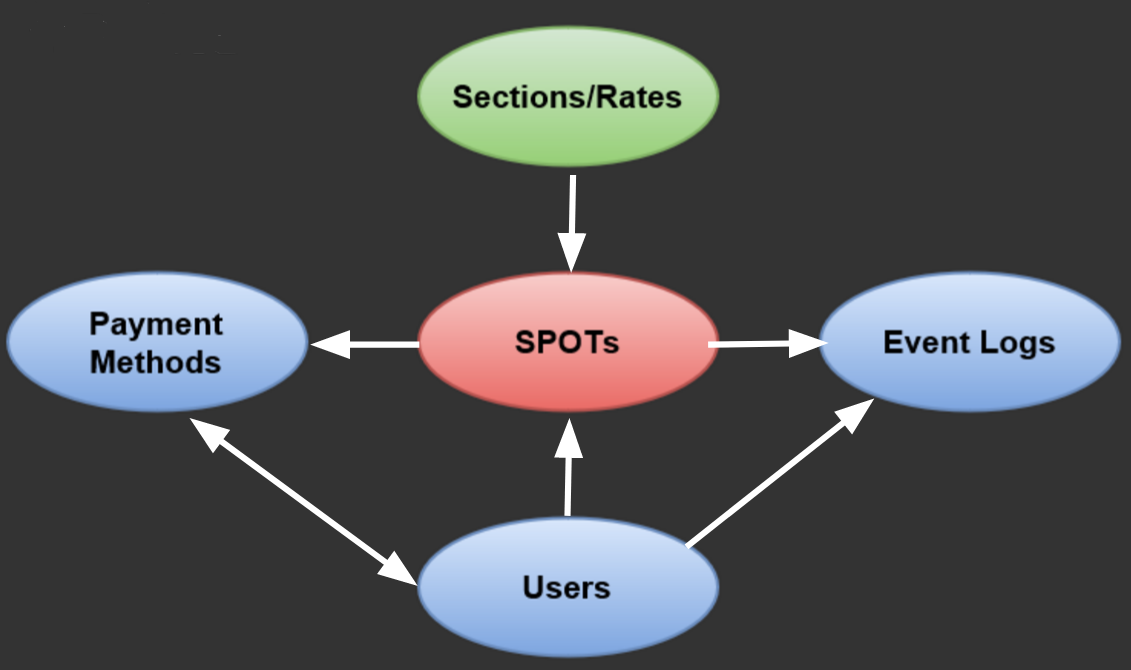
\includegraphics[width=0.85\textwidth]{pictures/models.png}
\caption{Relationships between database models.}
\end{figure}

In order to provide the basic functionality of knowing who parks where at what times, we need to keep track of two things: the SPOTs and the users.  
In addition to that we need an interface that lets us store pricing rate information, parking permit overrides, and historical logging for analytics.

\paragraph{SPOTs}
are the primary source of data in the system and maintain the "live" status of all sensors as well as some editable metadata about the SPOT.
\begin{lstlisting}[language=Python]
class spot_data(models.Model):
  uuid = models.UUIDField("UUID", 
      primary_key=True, unique=True)
  #"static" metadata about spot
  section = models.ForeignKey(sections, null=True)
  number = models.IntegerField("Spot Number")
  #"variable" current status
  last_update = models.DateTimeField("Last Update", 
      auto_now=True)
  occ_status = models.SmallIntegerField("Occupied Status", 
      default=0)
  occ_since = models.DateTimeField("Occupied Since")
  occ_license = models.CharField("Occupant License", 
      max_length=20)
  occupant = models.ForeignKey(Account, null=True)
class sections(models.Model):
  name = models.CharField("Section", max_length=100)
  structure = models.ForeignKey(structures, null=True)
  rates = models.TextField("Rates Array", 
      default=rates_default)
class structures(models.Model):
  name = models.CharField("Structure", max_length=100)
\end{lstlisting}
SPOTs have a UUID as a primary key so that each SPOT is easily identify-able and removing entries from the database is still extremely unlikely to produce duplicate identifiers.
The UUID is also 16 bytes, perfectly matching the Bluetooth beacon's UID size.  

SPOTs also contain some "static" geographic information about the SPOT such as a number, section, and lot.
These additional models are relatively minor themselves but allow each SPOT to be located and filtered based on its physical position.
SPOTs reference a Section that they belong in, which can be "level 1", "row A", etc.
Sections reference a Lot that they are part of, such as "West Core" or "Lot 151".

Lastly is the current live data about the SPOT: whether or not it's occupied and how long it's been in that state, who's parked there (if verification has occured) and any detected license plates.

\paragraph{User Accounts}
are necessary for drivers to register with the system so that SPOT knows who is parking where.
Luckily Django has a built-in interface for this which already provides login session management, registration, authentication, secure password storage, and other basic user account services.
In our current implementation we've only added a reference to payment methods that a user has purchased or authorized but future development will include being able to tie license plates and SPOT reservations to the user.
Currently there is not much we are using the User model for aside from all of the default functionality provided by Django; users are instead referenced by the other models and used to authenticate a driver.

\paragraph{Payment Methods}
are a list of permits and ways to be charged for parking.
\begin{lstlisting}[language=Python]
class payment_method(models.Model):
  name = models.CharField("Payment Method Name", 
      max_length=100)
  purchase_price = models.FloatField("Purchase Price", 
      default = 0.0)
  rate_modifier = models.FloatField("Rate Modifier", 
      default = 1.0)
\end{lstlisting}
Payment Methods can be thought of as an abstract class which can be extended to include credit cards, prepaid cards, old school tickets, or lot-specific parking permits as used by UCSC.
At the current stage of development they are almost a placeholder, only containing a purchase price and a "rate modifier".
This modifier is a basic percentage multiplier that is applied to the payment accrued while parking.

\paragraph{Event Logs}
are used to store the history of events that occur in the SPOT system.
\begin{lstlisting}[language=Python]
class event_log(models.Model):
  start = models.DateTimeField("Arrival", null=True)
  end = models.DateTimeField("Departure", null=True)
  total_paid = models.FloatField("Total charge", default=0)
  payment_method = models.ForeignKey(payment_method, 
      null=True)
  spot = models.ForeignKey(spot_data, null=True)
  user = models.ForeignKey(Account, null=True)
\end{lstlisting}
Each entry in the log is built to catalog everything about a driver's park in a SPOT.
When a SPOT detects an arrival a log entry is created with the SPOT being occupied and the time occupation began.
When verification occurs (either through license plate or Bluetooth) the log entry is updated to include the user account who was verified.
When a SPOT detects a departure the log entry updated with the time of departure, total amount paid, and payment used.

This catalog of events keeps the entire history of SPOTs available for future use.  The list of events can be filtered by a specific user account to provide a timeline or payment history.
It can also be filtered by SPOT, section, or lot for managers to calculate various usage analytics and display information on the web page.

\subsection{Payments}
SPOT allows lot managers to define hours of operation and parking rates in 15 minute increments across all seven days of the week.
This information is stored in a two-dimensional 7x96 float array where each value represents the hourly rate for that 15 minute interval.
Array indices and 24 hour times (00:00 - 23:59) can be determined with the following formulas:
\begin{equation}
    index = hour * 4 + \left \lfloor{minute / 15}\right \rfloor
\end{equation}
\begin{equation}
    hour = \left \lfloor{index / 4}\right \rfloor
\end{equation}
\begin{equation}
    minute = (index \% 4) * 15
\end{equation}
Index [0,0] represents Sunday from 00:00 to 00:15; [0,1] represents Sunday 00:15-00:30; [3,81] represents Wednesday 20:15-20:30; and so on.
Note that negative numbers are used to represent that the SPOT is unavailable att hat time.

Our current implementation calculates the total payment by building a rate mask of floats where each value is the percentage of the 15 minute interval that the SPOT was occupied.
That mask is then applied to the rate table for the SPOT's section, yielding an array whose values represent the amount owed for each 15 minute interval.
Summing all values in this array gives us the total amount owed, which is then multiplied by the rate modifier in the user's preferred payment method.

Future plans include redesigning this algorithm to improve reliability over multi-day parking and reduce overhead by instead walking through the time delta a SPOT was occupied and checking each applicable index in the array rather than building masks.

\subsection{Queries and Analytics}
Django's model interface allows database tables to be queried based on various field values, much like SQL.
For instance, all parking events for a user named "Daniel" can be retrieved and sorted by start time with the following code
\begin{lstlisting}[language=Python]
#get the user account for "Daniel"
Daniel_acc = Account.objects.filter(first_name='Daniel')[0]
#get the log entries associated with this account
Daniel_hist = event_log.objects.filter(user=Daniel_acc)
#sort them in decreasing order by the "start" field value
Daniel_sorted = Daniel_hist.order_by('-start')
\end{lstlisting}
Obtaining all of the SPOTs located on Level 1 of West Core is equally as simple:
\begin{lstlisting}[language=Python]
#get the lot named "West Core"
West_Core = lots.objects.filter(name='West Core')[0]
#get the "Level 1" section of West Core
WC_L1 = sections.objects.filter(lot=West_Core)[0]
#get the SPOTs in this section
WC_L1_SPOTs = spot_data.objects.filter(section=WC_L1)

#get SPOT 17, Level 1, West Core
WC_L1_17 = WC_L1_SPOTs.filter(number=17)[0]
\end{lstlisting}

Using Django's model interface allows us to perform complex database queries quickly and easily, allowing us to perform powerful analytics across multiple database tables.

%%%%%%%%%%%%%%%%%%%%%%%%%%
\newpage
\subsection{Front-end}
\subsubsection{Using Angular with Django}
Since we used Django Framework to to run our server, extra precautions were needed in order to avoid collisions with AngularJS syntax.
For example, to :
\vspace{0.5cm}
\begin{lstlisting}[language=html]

.
<p>{{ ang.binded_variable }}<\p>
.

\end{lstlisting}
\vspace{0.5cm}

Angular and Django are capable of binding data to HTML clientside and serverside, respectively.
Syntax collision occurs with angular bindings if they aren't wrapped in the code shown above.
This is because they both share data binding sytax of '{{ang.binded\_data}}'.
Pulling our github repository should set you up with the right structure.

\vspace{0.5cm}
\begin{figure}
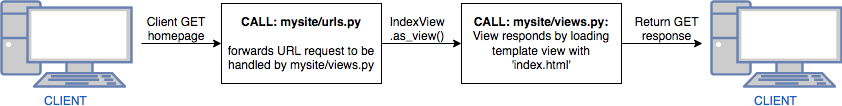
\includegraphics[width=1\textwidth]{pictures/Client_getIndex.png}
\caption{Sequence after a client requests the home page from our cloud server.}
\end{figure}

Next, let's load the home page.
Figure 10 shows a how the cloud server responds to a home page request.
Note how the Django View, different than ng-view, loads index.html into its response.
The django view gets handed HTTP requests and can deal with them as it wants.


\newpage
\subsubsection{Dynamic loading}
Responding with new HTML implies that the client should re-render, or refresh, their page.
To avoid unnecessary refreshes, we transferred new data through JSON files between server to client.
In this manner, we could communicate the addition of, for example, a new parking lot and have client-side AngularJS update the webpage seamlessly.
Instead of having to communicate new views via html, the server now encodes our data as JSON and Client-Side AngularJS decodes the json and updates the html view live.
This in an upcoming practice referred to as SPA (Single Page Application)

\vspace{0.5cm}
\begin{lstlisting}[language=html]
<div class="container-fluid">
		<div class="row">
			<div class="col-xs-12 ng-view"></div>
		</div
</div>
\end{lstlisting}
\vspace{0.5cm}

Angular allows directives to be integrated directly into HTML.
In this case, we use an ng-view element to dictate a dynamic HTML box in the DOM, that is the same size as the div it describes.
This becomes our dynamic environment wherein our AngularJS can dynamically update our home page HTML without re-rendering.
This includes having AngularJS dynamically inject entire HTML pages.

\begin{figure}
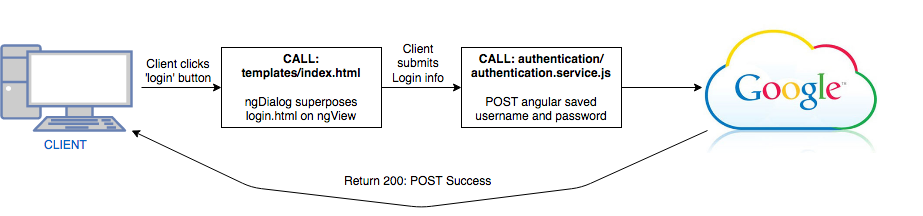
\includegraphics[width=1\textwidth]{pictures/Client_angRouting(2).png}
\caption{Sequence after a client requests the home page from our cloud server.}
\end{figure}

\newpage
\subsection{Website}
\subsubsection{Monitor}
\begin{figure}[htb]
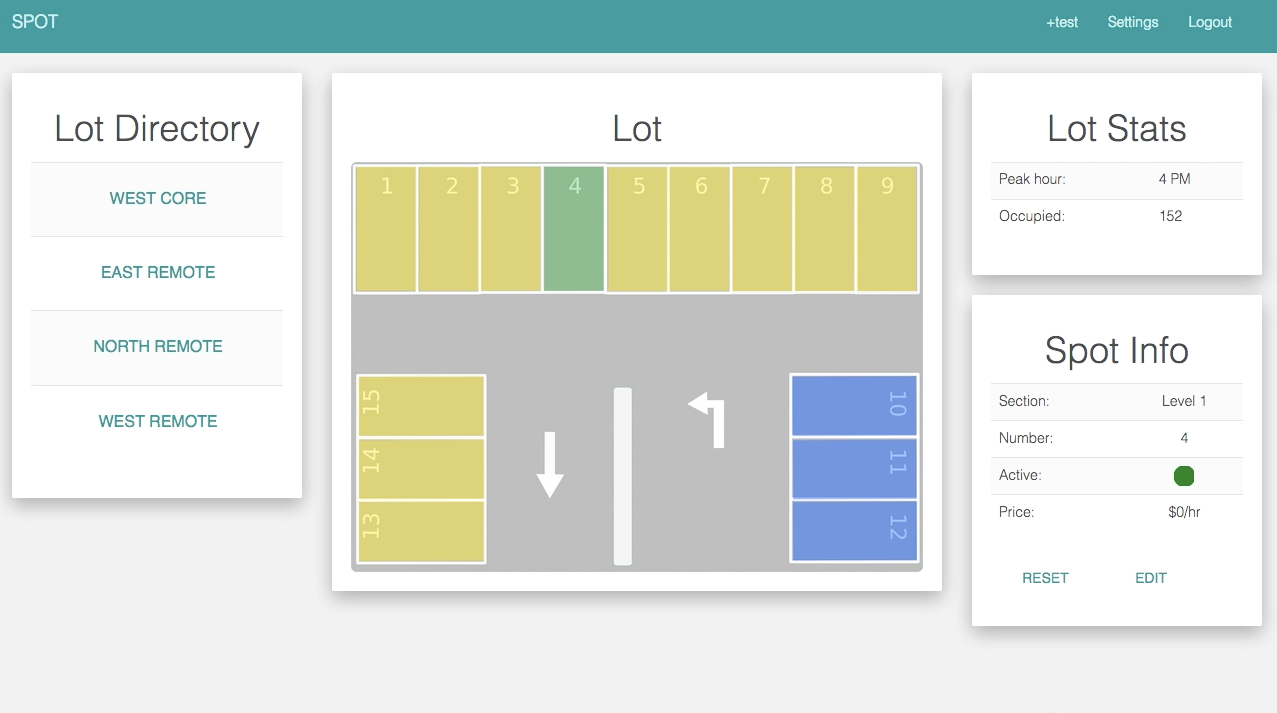
\includegraphics[width=1\textwidth]{pictures/MonitorScreen.png}
\caption{Screen shot of the finished monitor page.}
\end{figure}

After downloading a Django template project, you should find that there's a particular directory structure.
Note that django has a modular manner of splitting up large/related tasks into 'apps'.
For instance, we had an app 'monitor' which housed all the django python and html templates that related to our monitor page.
There are two main ways of returning a page. One can use Django URL routing (See django/monitor/urls.py) or by using the using Angular routers hooked with Django (See django/static/javascripts/sdpspot.routes.js).
The former can only modify HTML before sending it off to the client, while the latter can modify HTML after being received by the client.
Using angular routing, we developed a Web API that allowed us to SPA-update the user's page with info from our database:


\newpage
\begin{table}[!htb]
\renewcommand{\arraystretch}{1}
\centering
\caption{Client-Side Web API}
\begin{tabular}{|c||c|c|}
\hline
\textbf{Function Call} & \textbf{Method} & \textbf{Description} \\
\hline
/api/v1/monitor/list\_sections/ & GET & Returns list of parking sections \\
\hline
/api/v1/monitor/list\_lots/ & GET & Returns list of parking lots \\
\hline
/api/v1/monitor/list\_spots/ & GET & Returns list of parking spots \\
\hline

\end{tabular}
\end{table}

This Web API returns objects that describe sections, lots, and SPOTs.
Inside these objects, all relevant data is we receive all relevant data from the server and incorporate it into our client side Javascript.
Great, we've successfully gotten our data from the server, however if we want our page to stay up to date we need to periodically request this data.

\vspace{0.5cm}
\begin{lstlisting}[language=JavaScript]
function load_periodic() {
      setInterval(function() {
        load_spots();
        load_sections();
      }, 1250);
}
\end{lstlisting}




\newpage
\subsection{Phone Application}
%%%%%%%%%%%%%%%%%%%%%%
\begin{figure}
\centering
\begin{subfigure}{.4\textwidth}
  \centering
  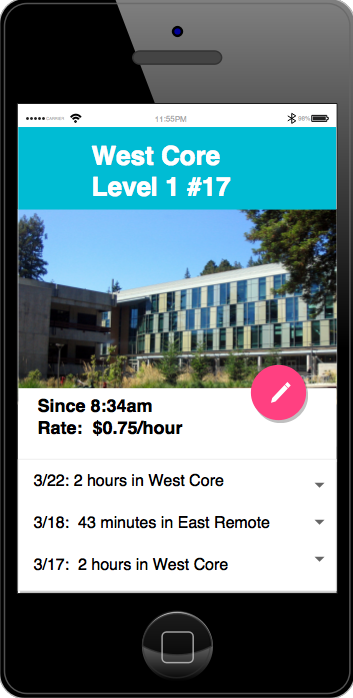
\includegraphics[width=.55\linewidth]{pictures/phone.png}
  \caption{Screen shot of the phone's redirect page to /mobile.}
%   \label{fig:3dprinted}
\end{subfigure}%
\hspace{1cm}
\begin{subfigure}{.4\textwidth}
  \centering
  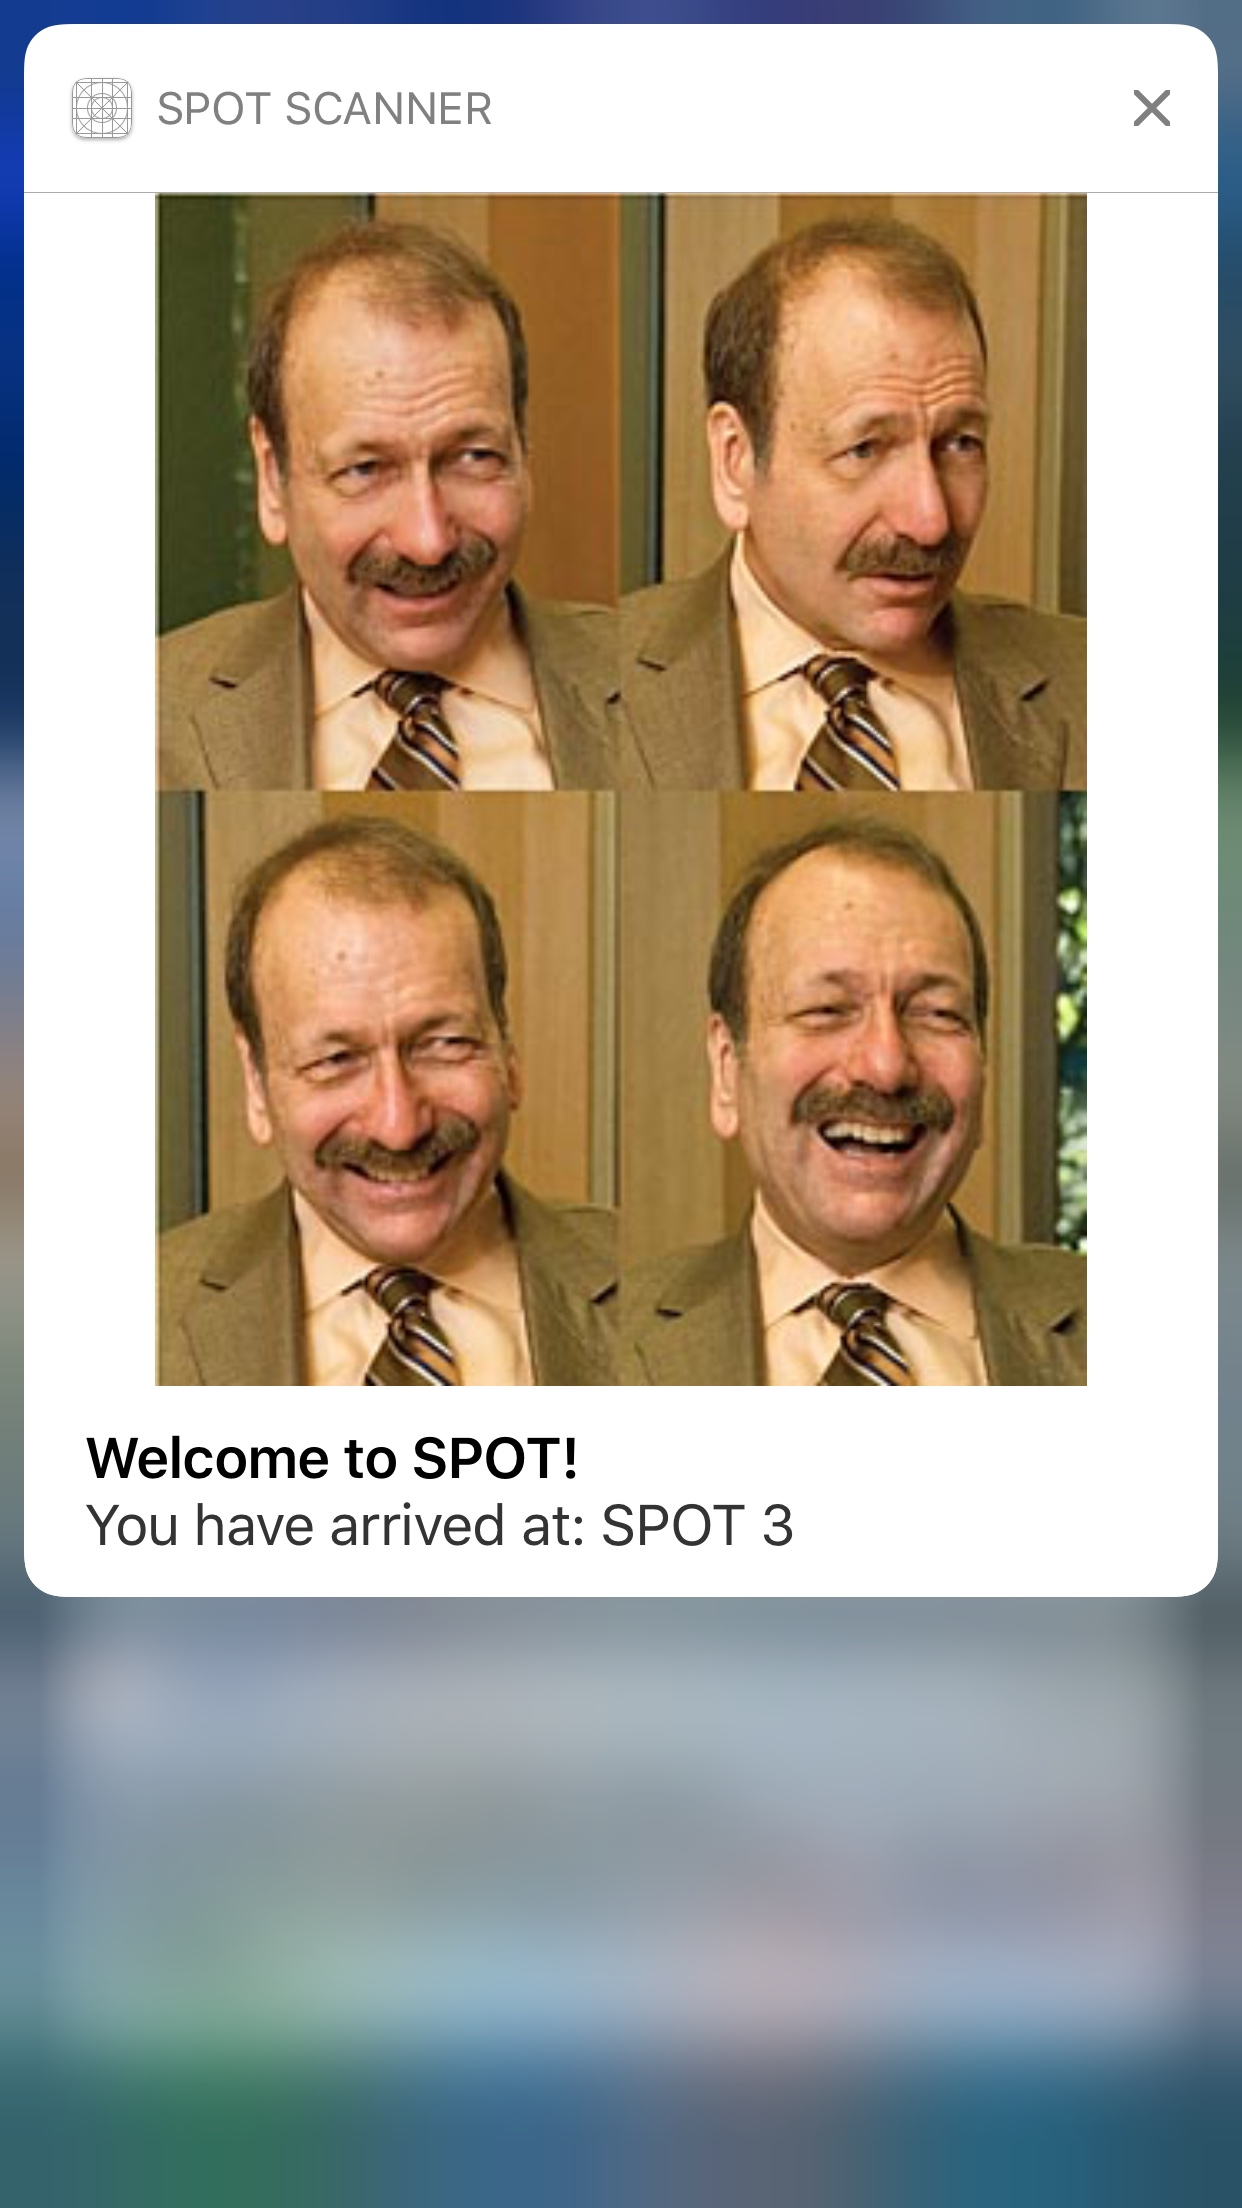
\includegraphics[width=0.6\linewidth]{pictures/blummy.jpeg}
  \caption{Screen shot of phone's notification upon arrival.}
%   \label{fig:acrylictube}
\end{subfigure}
\caption{Representation of what the driver would see on their phone.}
% \label{fig:test}
\end{figure}
%%%%%%%%%%%%%%%%%%%%%
We successfully made an Android and iOS app that was able to pick up eddystone beacons.
The app was dependent on the tutorial found from \textit{Github}\footnote{https://github.com/google/eddystone}.
Sequentially from the beacon detection, we redirected our app to our website's mobile page.
Instantaneously the server is notified that a user has arrived at a specific SPOT in our system.
To establish connection with the database, the drive must be logged in and verified by Django's authentication system.
For iOS development, you can open NSURL sessions that allows us to request verification from the server.
\begin{lstlisting}[language=C]
[[session_login dataTaskWithRequest:request_login completionHandler:
        ^(NSData *data, NSURLResponse *response, NSError *error) {
        NSString *requestReply = [[NSString alloc] initWithData:data 
                                encoding:NSASCIIStringEncoding];
        NSLog(@"requestReply_login: %@", requestReply);
}] resume];
\end{lstlisting}
Through the data received on the app, we implement a JSON parser for targeting details on what the SPOT number is as well as details such as parking rates.
% NSError *e = nil;
% NSArray *JSONarray = [NSJSONSerialization JSONObjectWithData: data options: NSJSONReadingMutableContainers error: &e];
\begin{lstlisting}[language=C]
for(int i=0;i<[JSONarray count];i++)
{
    spot_number = [[JSONarray objectAtIndex:i]objectForKey:@"number"]);
}
\end{lstlisting}
Using this sample of Objective-C we were able to implement the built in JSON parser to isolate the exact spot number correlated with the database.
With the information given from the database, the app ties the user's account with \textit{SPOT 4}, and the server stamps their arrival time immediately to automate billing.
Next, the app redirects to a URL when a beacon was detected. 
This forwards the information from the beacon to the phone, then from the phone to the cloud, from the cloud back to the phone as shown in the Figure 3. 
This is how the data is given to the cloud from the driver's phone.
With the URL that was redirected from the app, the user will eventually be able to authenticate themselves with a user login/sign up web page. 
Users can confirm the parking spot they parked in and pay through the app rather than a pay station.  
